\section{Continued use of Scrum}
Group work, especially pair-programming was very important to bring the individual code contributions together. However, the hours of work time spent on the last submission were not distributed as evenly as was the case for the previous submissions as the number of hours increased exponentially during the last 2 weeks before the deadline.
\subsection{Sprints}

\begin{figure}[h]
	\centering
	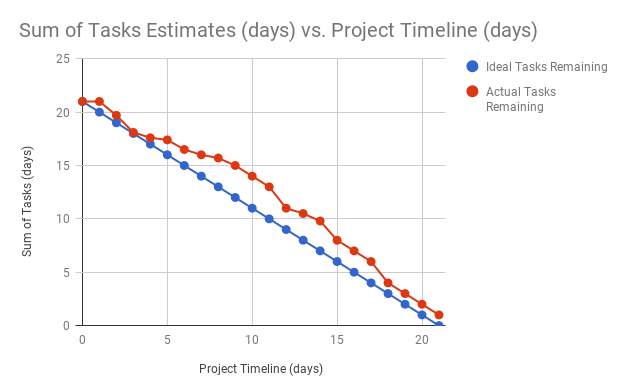
\includegraphics[width=0.6\textwidth]{burndown}
	\caption{A Burndown Chart for the past 14 days.}\label{fig:burn}
\end{figure}
The short time period of 2 weeks meant that we decided to have only 1 sprint and no more role-rotations until the final deadline. During these 2 weeks we met up almost every day to discuss individual task assignments, asses our sprint progress and work on tasks jointly. Although the tasks identified from the initial specifications were not completed to their entirety as discussed earlier, all feasible work was completed in time and progress was made throughout the time period of the sprint.
\subsection{Scrum board}
Again, the scrum board was used to outline and track the completion of each task. The same whiteboard in the John Honey main computer lab was used in order to maintain consistency. This gave a clear visual representation of the objectives. During the sprint, the main jobs required for completion were to further enhance the testing unit to increase its coverage across the implemented systems, implement a simple file converter and introduce a logging system for the server. Much experience was gained from completing previous sprints and so using this experience we were better equipped to handle larger tasks. Examples of the board in use can be found in Appendix \ref{app:board}.

\subsection{Meetings}
Regular meetings were also held to discuss and evaluate progress. This was crucial in the scrum process and as working in a team to allow a point of communication between each member at the same point in time. An example of a major decision being made during the discussion was the change of language of the file converter implementation. It was decided that the more appropriate language to use would be C as there would more extensive libraries for this particular operation and would also have the advantage of greater efficiency. Multiple meetings were held during the most recent sprint to determine the tasks required for completion, to evaluate whether each task was completed and track progress in between.
The minutes for formal meetings are available in Appendix \ref{app:meet}.
